\section{Potenzialfelder und Mehrfachintegrale}

\begin{ejercicio}[Kurvenintegral einer Funktion mit Potenzial]

    Im $\bb{R}^2$ ist eine Kurve gegeben durch die Parameterdarstellung
    \Func{\varphi}{\left[0, \nicefrac{\pi}{2}\right]}{\bb{R}^2}{t}{\left(\sin t, t\right)}

    Berechnen Sie das Kurvenintegral $\displaystyle \int_{\varphi} \vec{f} \cdot d\vec{s}$ für:
    \Func{\vec{f}}{\bb{R}^2}{\bb{R}^2}{(x,y)}{\begin{pmatrix}
2xy + 2\cos(y) \\ x^2 - 2x\sin(y) + 1
    \end{pmatrix}}
    \begin{observacion}
        Prüfen Sie, ob $\vec{f}$ ein Potenzial hat und nutzen Sie es ggf. aus.
    \end{observacion}

    Let's first check that $\varphi$ is a regular parametrization:
    \[\varphi'(t) = (\cos t, 1) \]
    Given that $1\neq 0$ for all $t \in \left[0, \nicefrac{\pi}{2}\right]$, we conclude that $\varphi$ is regular.
    Let's now try to calculate the integral directly. In order to do so, we need to compute $\vec{f}(\varphi(t))\cdot \varphi'(t)$:
    \begin{align*}
        \vec{f}(\varphi(t)) &= \vec{f}(\sin t, t) = \begin{pmatrix}
            2\sin t \cdot t + 2\cos t \\
            \sin^2 t - 2\sin^2 t + 1
        \end{pmatrix} = \begin{pmatrix}
            2t \sin t + 2\cos t \\
            1 - \sin^2 t
        \end{pmatrix} = \begin{pmatrix}
            2t \sin t + 2\cos t \\
            \cos^2 t
        \end{pmatrix} \\
        \varphi'(t) &= (\cos t, 1) \\
        \vec{f}(\varphi(t))\cdot \varphi'(t) &= 2t \sin t \cos t + 2\cos^2 t + \cos^2 t = 2t \sin t \cos t + 3\cos^2 t
    \end{align*}

    Therefore, the integral is:
    \begin{align*}
        \int_{\varphi} \vec{f} \cdot d\vec{s} &= \int_0^{\nicefrac{\pi}{2}} \left( 2t \sin t \cos t + 3\cos^2 t \right) dt
    \end{align*}

    Given that integrating this expression is quite cumbersome, let's check if $\vec{f}$ has a potential function. Given that $\bb{R}^2$ is star-shaped, we check:
    \begin{align*}
        \dfrac{\partial f_1}{\partial y} &= 2x - 2\sin(y) \\
        \dfrac{\partial f_2}{\partial x} &= 2x - 2\sin(y)
    \end{align*}

    Since the mixed partial derivatives are equal, $\vec{f}$ has a potential function. Let's find it:
    \begin{description}
        \item[Option 1] Having fixed $(x,y)\in \bb{R}^2$, let's consider the following path from $(0,0)$ to $(x,y)$:
        \Func{\Phi}{[0,1]}{\bb{R}^2}{t}{(tx, ty)}
        
        Let's also write the potential function as $u: \bb{R}^2 \to \bb{R}$. Then:
        \begin{align*}
            \int_{\Phi} \vec{f} \cdot d\vec{s} &= u(\Phi(1)) - u(\Phi(0)) = u(x,y) 
            \Longrightarrow u(x,y) = \int_0^1 \vec{f}(\Phi(t)) \cdot \Phi'(t) dt + u(0,0)
        \end{align*}

        Given that the potential is defined up to a constant, we can set $u(0,0) = 0$. Now, let's compute $\vec{f}(\Phi(t)) \cdot \Phi'(t)$:
        \begin{align*}
            \vec{f}(\Phi(t)) &= \vec{f}(tx, ty) = \begin{pmatrix}
                2(tx)(ty) + 2\cos(ty) \\
                (tx)^2 - 2(tx)\sin(ty) + 1
            \end{pmatrix} = \begin{pmatrix}
                2t^2 xy + 2\cos(ty) \\
                t^2 x^2 - 2tx \sin(ty) + 1
            \end{pmatrix} \\
            \Phi'(t) &= (x, y) \\
            \vec{f}(\Phi(t)) \cdot \Phi'(t) &= 2t^2 x^2y + 2x\cos(ty) + t^2 x^2y - 2txy \sin(ty) + y \\
            &= 3t^2 x^2y + 2x\cos(ty) - 2txy \sin(ty) + y
        \end{align*}

        Therefore, the potential function is:
        \begin{align*}
            u(x,y) &= \int_0^1 \left( 3t^2 x^2y + 2x\cos(ty) - 2txy \sin(ty) + y \right) dt
            =\\&= \left[ x^2 y t^3 + \dfrac{2x}{y} \sin(ty) +yt\right]_0^1 -2xy\int_0^1 t \sin(ty) dt
            =\\&= x^2 y + \dfrac{2x}{y} \sin(y) + y - 2xy \int_0^1 t \sin(ty) dt
        \end{align*}

        To compute the remaining integral, we use integration by parts:
        \begin{equation*}
            \MetInt{u(t)=t\qquad u'(t)=1}{v(t)=-\dfrac{1}{y}\cos(ty) \qquad v'(t)=\sin(ty)}
        \end{equation*}
        \begin{align*}
            \int_0^1 t \sin(ty) dt &= \left[ -\dfrac{t}{y} \cos(ty) \right]_0^1 + \dfrac{1}{y} \int_0^1 \cos(ty) dt
            =\\&= \left[ -\dfrac{t}{y} \cos(ty) + \dfrac{1}{y^2} \sin(ty) \right]_0^1
            = -\dfrac{1}{y} \cos(y) + \dfrac{1}{y^2} \sin(y)
        \end{align*}

        Therefore, the potential function is:
        \begin{align*}
            u(x,y) &= x^2 y + \dfrac{2x}{y} \sin(y) + y - 2xy \left( -\dfrac{1}{y} \cos(y) + \dfrac{1}{y^2} \sin(y) \right)
            =\\&= x^2 y + \cancel{\dfrac{2x}{y} \sin(y)} + y + 2x \cos(y) - \cancel{\dfrac{2x}{y} \sin(y)}
            =\\&= x^2 y + y + 2x \cos(y)
        \end{align*}
        \item[Option 2] 
        
        We look for a function $u(x,y)$ such that:
        \begin{align*}
            \dfrac{\partial u}{\partial x} &= 2xy + 2\cos(y) \\
            \dfrac{\partial u}{\partial y} &= x^2 - 2x\sin(y) + 1
        \end{align*}

        Integrating the first equation with respect to $x$:
        \begin{align*}
            u(x,y) &= \int 2xy + 2\cos(y) \, dx = x^2 y + 2x \cos(y) + h(y)
        \end{align*}
        where $h(y)$ is an arbitrary function of $y$. Now, we differentiate $u(x,y)$ with respect to $y$ and equate it to the second equation:
        \begin{align*}
            \dfrac{\partial u}{\partial y} &= x^2 - 2x \sin(y) + h'(y) = x^2 - 2x \sin(y) + 1
            \Longrightarrow h'(y) = 1 \Longrightarrow h(y) = y + C
        \end{align*}

        Given that the potential is defined up to a constant, we can set $C=0$. Therefore, the potential function is:
        \begin{align*}
            u(x,y) = x^2 y + 2x \cos(y) + y
        \end{align*}
    \end{description}

    Finally, we can compute the integral using the potential function:
    \begin{align*}
        \int_{\varphi} \vec{f} \cdot d\vec{s} &= u(\varphi(\nicefrac{\pi}{2})) - u(\varphi(0)) = u(1, \nicefrac{\pi}{2}) - u(0,0) = \dfrac{\pi}{2} + 2\cos(\nicefrac{\pi}{2}) + \frac{\pi}{2} - 0 = \pi
    \end{align*}
\end{ejercicio}


\begin{ejercicio}[Doppelintegral mit e-Funktion]
    Berechnen Sie
    \begin{equation*}
    I = \int_0^1 \int_0^{y^2} e^{\nicefrac{x}{y}} \, dx \, dy
    \end{equation*}
    \begin{align*}
        \int_0^{1} \int_0^{y^2} e^{\nicefrac{x}{y}} \, dx \, dy &= \int_0^1 \left[ y e^{\nicefrac{x}{y}} \right]_0^{y^2} dy = \int_0^1 y \left( e^y - 1 \right) dy = \int_0^1 y e^y dy - \int_0^1 y dy
    \end{align*}

    To compute the remaining integral, we use integration by parts:
    \begin{equation*}
        \MetInt{u(y)=y\qquad u'(y)=1}{v(y)=e^y \qquad v'(y)=e^y}
    \end{equation*}
    \begin{align*}
        \int_0^1 y e^y dy &= \left[ y e^y \right]_0^1 - \int_0^1 e^y dy = \left[ y e^y - e^y \right]_0^1 = (e - e) - (0 - 1) = 1
    \end{align*}

    Therefore, the value of the integral is:
    \begin{align*}
        I &= 1 - \left[ \dfrac{y^2}{2} \right]_0^1 = 1 - \dfrac{1}{2} = \dfrac{1}{2}
    \end{align*}
\end{ejercicio}


\begin{ejercicio}[Flächenberechnung mit Doppelintegral]\label{ej:10.3}
    Ein Flächenstück wird durch die Kurven $x=0$, $y=2x$ $y=\nicefrac{1}{a}x^2 + a$, $a > 0$ berandet.
    Berechnen Sie den Flächeninhalt $A$ mit Hilfe eines Doppelintegrals.

    \begin{figure}
        \centering
        \begin{tikzpicture}
            \begin{axis}[
                axis lines = middle,
                xlabel = {$x$},
                ylabel = {$y$},
                clip=true,
                axis equal,
            ]

            \def\a{1.5}
            % Definir el color naranja
            \definecolor{myorange}{HTML}{FFA500}

            % Para que la función `fill between` funcione, las parcelas deben tener nombres
            % Modifica tus addplot existentes así:
            \addplot [
                domain=-1:2, 
                samples=100,
                blue,
                name path=parabola_plot % Añade un nombre
            ]{(1/\a)*x^2 + \a};
            \addlegendentry{$y=\frac{1}{a}x^2 + a$}

            \addplot [
                domain=0:2, 
                samples=2,
                red,
                name path=line_plot % Añade un nombre
            ]{2*x};
            \addlegendentry{$y=2x$}

            % Rellenar el área entre la parábola y la recta de 0 a 1.5
            \addplot [
                thick,
                color=orange,
                fill=orange,
                fill opacity=0.4
            ]
            fill between [
                of=parabola_plot and line_plot,
                soft clip={domain=0:1.5},
            ];
            \addlegendentry{$A$}
            \end{axis}
        \end{tikzpicture}
        \caption{Area to be calculated in Exercise~\ref{ej:10.3}.}
        \label{fig:area_ej_10_3}
    \end{figure}

    In Figure~\ref{fig:area_ej_10_3}, we can see the area to be calculated. Let's first find the points of intersection between the curves $y=2x$ and $y=\nicefrac{1}{a}x^2 + a$:
    \begin{align*}
        2x &= \dfrac{1}{a}x^2 + a
        \Longrightarrow x^2 - 2ax + a^2 = 0
        \Longrightarrow (x - a)^2 = 0
        \Longrightarrow x = a
    \end{align*}
    Therefore, the curves intersect at the point $(a, 2a)$. Given that the area is bounded by $x=0$ and $x=a$, we can set up the double integral to calculate the area:
    \begin{align*}
        A &= \int_0^a \int_{2x}^{\nicefrac{1}{a}x^2 + a} dy \, dx = \int_0^a \left( \dfrac{1}{a}x^2 + a - 2x \right) dx = \left[ \dfrac{1}{3a}x^3 + ax - x^2 \right]_0^a =\\&= \dfrac{1}{3a}a^3 + a^2 - a^2 - 0 = \dfrac{a^2}{3}
    \end{align*}
\end{ejercicio}

\begin{ejercicio}[Flächeninhalt mit Polarkoordinaten]
    \label{ej:10.4}
    Die Randkurve eines Gebiets in der Ebene wird durch die Gleichung
    \[r = 2(\cos(\varphi) + \sin(\varphi))\]
    in Polarkoordinaten beschrieben. Berechnen Sie den Flächeninhalt $A$ dieses Gebiets.

    \begin{figure}
        \centering
        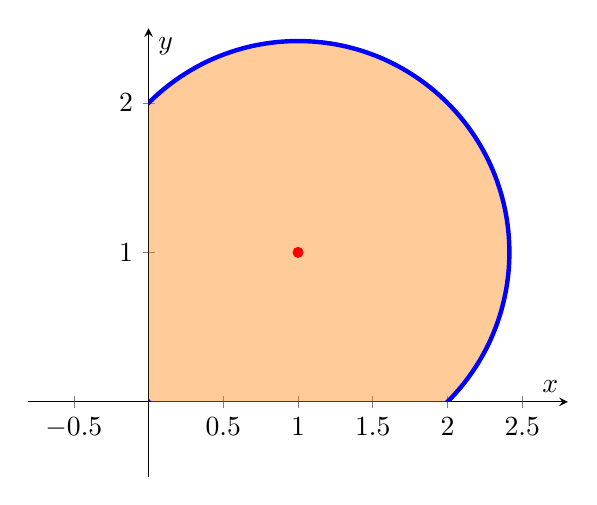
\begin{tikzpicture}
            \begin{axis}[
                % Configuración de los ejes
                axis lines=middle,
                xlabel=$x$,
                ylabel=$y$,
                xmin=-0.5, xmax=2.5,
                ymin=-0.5, ymax=2.5,
                % Ajustar la relación de aspecto para que el círculo se vea redondo
                axis equal
            ]

            \clip (axis cs:0,0) rectangle (axis cs:2.5, 2.5);

            % 1. Rellenar el área A (El círculo)
            % Usamos la función \draw con fill. 
            % El centro es (1, 1) y el radio es sqrt(2) ≈ 1.414.
            \draw[fill=orange, opacity=0.4, draw=none] (axis cs:1, 1) circle ({sqrt(2)});

            % 2. Dibujar el borde de la curva (El círculo)
            \draw[blue, ultra thick] (axis cs:1, 1) circle ({sqrt(2)});
            
            % 3. Marcar el centro del círculo (1, 1)
            \fill[red] (axis cs:1, 1) circle (2pt);

            \end{axis}
        \end{tikzpicture}
        \caption{Area to be calculated in Exercise~\ref{ej:10.4}.}
        \label{fig:area_polar_ej}
    \end{figure}

    In Figure~\ref{fig:area_polar_ej}, we can see the area to be calculated. Using polar coordinates, the area can be calculated as:
    \begin{align*}
        A &= \int_0^{\nicefrac{\pi}{2}} \int_0^{2(\cos(\varphi) + \sin(\varphi))} r \, dr \, d\varphi = \int_0^{\nicefrac{\pi}{2}} \left[ \dfrac{r^2}{2} \right]_0^{2(\cos(\varphi) + \sin(\varphi))} d\varphi = \int_0^{\nicefrac{\pi}{2}} 2(\cos(\varphi) + \sin(\varphi))^2 d\varphi
        =\\&= 2 \int_0^{\nicefrac{\pi}{2}} \left( \cos^2(\varphi) + 2\sin(\varphi)\cos(\varphi) + \sin^2(\varphi) \right) d\varphi = 2 \int_0^{\nicefrac{\pi}{2}} \left( 1 + \sin(2\varphi) \right) d\varphi
        =\\&= 2 \left[ \varphi - \dfrac{1}{2} \cos(2\varphi) \right]_0^{\nicefrac{\pi}{2}} = 2 \left( \dfrac{\pi}{2} - \dfrac{1}{2} \cos(\pi) - \left(0 - \dfrac{1}{2} \cos(0)\right) \right) = 2 \left( \dfrac{\pi}{2} + \dfrac{1}{2} + \dfrac{1}{2} \right) = \pi + 2
    \end{align*}
\end{ejercicio}

\begin{ejercicio}[Dreifachintegral in Zylinderkoordinaten]
    Berechnen Sie das folgende in Zylinderkoordinaten gegebene Integral:
    \[
    I = \int_{\pi}^{2\pi} \int_0^1 \int_{r}^{r^2}rz \cdot \sin(\varphi) \, dz \, dr \, d\varphi.
    \]
    \begin{align*}
        I&= \int_{\pi}^{2\pi} \int_0^1 \int_{r}^{r^2} rz \sin(\varphi) \, dz \, dr \, d\varphi = \int_{\pi}^{2\pi} \int_0^1 \left[ \dfrac{rz^2}{2} \sin(\varphi) \right]_{z=r}^{z=r^2} dr \, d\varphi
        =\\&= \int_{\pi}^{2\pi} \sin(\varphi) \int_0^1 r\cdot \left[\dfrac{z^2}{2}\right]_{r}^{r^2} dr \, d\varphi = \int_{\pi}^{2\pi} \sin(\varphi) \int_0^1 r \cdot \left( \dfrac{r^4}{2} - \dfrac{r^2}{2} \right) dr \, d\varphi
        =\\&= \dfrac{1}{2}\int_{\pi}^{2\pi} \sin(\varphi) \int_0^1 \left( r^5 - r^3 \right) dr \, d\varphi = \dfrac{1}{2} \int_{\pi}^{2\pi} \sin(\varphi) \left[ \dfrac{r^6}{6} - \dfrac{r^4}{4} \right]_0^1 d\varphi
        =\\&= \dfrac{1}{2} \int_{\pi}^{2\pi} \sin(\varphi) \left( \dfrac{1}{6} - \dfrac{1}{4} \right) d\varphi = -\dfrac{1}{24} \int_{\pi}^{2\pi} \sin(\varphi) d\varphi = \dfrac{1}{24} \left[ \cos(\varphi) \right]_{\pi}^{2\pi} = \dfrac{1}{24} (1 - (-1)) = \dfrac{1}{12}
    \end{align*}
\end{ejercicio}